\documentclass{standalone}
\usepackage{tikz}
\usetikzlibrary{arrows}
\tikzset{
	treenode/.style = {align=center, inner sep=2pt, text centered},
	n/.style = {treenode, circle, draw,text width=2em}
}

\begin{document}
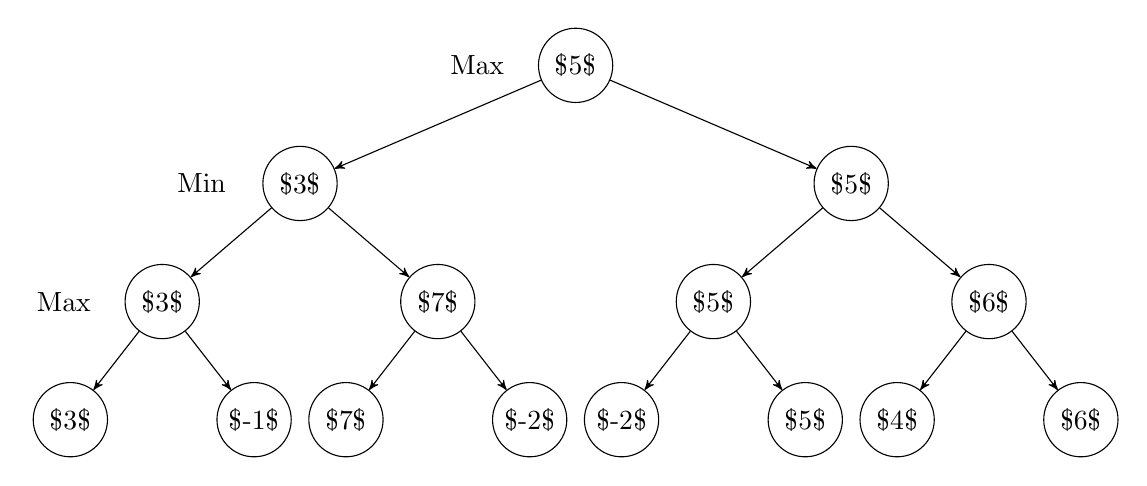
\begin{tikzpicture}[->,>=stealth',level/.style={sibling distance = 7cm/#1, level distance = 1.5cm}]
	\node [n] {\$5\$}
		child{node[n] {\$3\$}
			child{ node[n] {\$3\$}
				child{ node[n] {\$3\$}
				}
				child{ node[n] {\$-1\$}
				}
			}
			child{ node[n] {\$7\$}
				child{ node[n] {\$7\$}
				}
				child{ node[n] {\$-2\$}
				}
			}
		}
		child{ node[n] {\$5\$}
			child{ node[n] {\$5\$}
				child{ node[n] {\$-2\$}
				}
				child{ node[n] {\$5\$}
				}
			}
			child{ node[n] {\$6\$}
				child{ node[n] {\$4\$}
				}
				child{ node[n] {\$6\$}
				}
			}
		};
	\node[] (t1) at (-1.25,0) {Max};
	\node[] (t2) at (-4.75,-1.5) {Min};
	\node[] (t3) at (-6.5,-3) {Max};
	\end{tikzpicture}
\end{document}
